\documentclass[dvipsnames, 12pt]{article}
\usepackage{geometry}
\geometry{scale=0.75}
\usepackage{amsmath, amsthm, amssymb, bm, color, framed, tikz}
\usepackage{algorithm}
\usepackage[noend]{algpseudocode}
\bibliographystyle{plain} 
\usepackage[hypertexnames=false, colorlinks=true]{hyperref}

% Custom options for hyperlink colors or styles
\hypersetup{
    colorlinks=true,
    linkcolor=blue,       % Color for internal links (e.g., equations, sections)
    citecolor=red,        % Color for citations
    urlcolor=ForestGreen, % Color for URLs
    linktocpage=true      % Makes the TOC links point to the page number instead of the section title
}


\usepackage{tcolorbox}
\tcbuselibrary{skins}

\newcounter{problemcounter} % Define a new counter

\newtcolorbox{problem}[1]{%
    enhanced,
    colback=yellow!10!white,
    colframe=OliveGreen,
    fonttitle=\bfseries,
    title={Problem \refstepcounter{problemcounter}\theproblemcounter #1}, % Use the counter in the title
    attach boxed title to top left={yshift=-3mm,xshift=3mm},
    boxed title style={size=small,colback=OliveGreen!50!white}
}

% Commonly used sets
\newcommand{\Z}{\mathbb{Z}}
\newcommand{\RR}{\mathbb{R}}
\newcommand{\C}{\mathbb{C}}
\newcommand{\Q}{\mathbb{Q}}
\newcommand{\N}{\mathbb{N}}
\newcommand{\uu}{\mathbf{u}}

% Mathematical theorem, lemma, etc.
\newtheorem{Theorem}{Theorem}[section]
\newtheorem{Lemma}[Theorem]{Lemma}
\newtheorem{Corollary}[Theorem]{Corollary}
\newtheorem{Definition}[Theorem]{Definition}
\newtheorem{Example}[Theorem]{Example}
\newtheorem{Proposition}[Theorem]{Proposition}
\newtheorem{Conjecture}[Theorem]{Conjecture}
\newtheorem{Remark}[Theorem]{Remark}

\begin{document}



\section{Matrix-Vector Multiplication}


\paragraph{Coordinate Representation.} If we write $b$ as $A(A^{-1}b)$, one can see that $A^{-1}b$ is exactly the coefficient of expansion of $b$ in the basis of $A$.

\paragraph{Geometric representation.} We can view $Ax$ as $\operatorname{range}(A)$, i.e. subspace spanned by column vectors $a_{1}, a_{2}, \cdots, a_{n}$. If vector $b$ is perpendicular to this subspace, one has $A^{T} b =0$, which corresponds to $\langle a_{i}, b\rangle = a_{i}^{T} b =0$.

\begin{problem}{}
     By considering what space is spanned by the first $n$ columns of $R$ and using (1.8), show that if $R$ is a nonsingular $m \times m$ upper-triangular matrix, then $R^{-1}$ is also upper-triangular. (The analogous result also holds for lower-triangular matrices.)
\end{problem}

\begin{proof}
    This is a simple extension of solving upper triangle system
    $$
    Rx = b
    $$
    and when we consider appropriate $b$'s, saying
    $$
    R[x_{1}, x_{2}, \cdots, x_{n}] = [\delta_{1}, \delta_{2}, \cdots, \delta_{n}]
    $$
    One can see $x_{ij} = 0$ when $i<j$ since the first $i$ columns of $R$ is spanned by $[\delta_{1},\cdots, \delta_{i}]$.
\end{proof}

One of the most important transformations is projection and let's start with simple example-projection of vector $v$ to unit $q$. Assume we move both vectors at origin and the projection length is the inner product of two vectors $q^{*}v$ (minus sign means the angle between them is greater than $\pi/2$). Hence the projection is $(q^{*}v) q$, which can be also rewritten as $(qq^{*})v$ through the lens of transformation $qq^{*}$.

Think what remains about $v$ after subtracting the projection part $(q^{*}v) q$? If we decompose the Euclidean space into $H\oplus q$, then it's clear that $v-(q^{*}v) q$ falls into the subspace $H$ which can be seen as a hyperplane orthogonal to $q$. Moreover, one can see that $v-2(q^{*}v)q$ is exactly the image of $v$ in the \textbf{mirror} $H$.

An isometric transformation from $v$ to $w$ originates from \textbf{reflection} through the hyperplane $H$ which is orthogonal to $v-w$!

\begin{problem}{}
    Suppose $a, b$ are column vectors in $\mathbb{R}^n$ and they are orthogonal, please investigate $M: = ab^{T} + ba^{T}$.
\end{problem}

Geometrically, it can be interpreted as a reflection within the plane spanned by $a$ and $b$, combined with a scaling.

Let's consider the action of $M$ on a vector $x \in \mathbb{R}^n$: $Mx = ab^Tx + ba^Tx$.  The term $ab^Tx$ projects $x$ onto $b$ (along the direction of $b$), then becomes a scalar to dilate vector $a$. 

Because $a$ and $b$ are orthogonal, these projections are independent. The transformation effectively exchanges the components of $x$ along $a$ and $b$. If $\|a\| = \|b\|$, the transformation is a pure reflection in the hyperplane orthogonal to both $a$ and $b$.  If $\|a\| \neq \|b\|$, a scaling is also involved.


\begin{Example}
    \label{example04}
    \begin{enumerate}
        \item Let $a = \begin{bmatrix} 1 \\ 0 \\ 0 \end{bmatrix}$       and $b = \begin{bmatrix} 0 \\ 1 \\ 0\end{bmatrix}$. Then

            $$
            ab^T + ba^T = \begin{bmatrix} 0 & 1 & 0 \\ 0 & 0 & 0 \\ 0 & 0 & 0 \end{bmatrix} + \begin{bmatrix} 0 & 0 & 0 \\ 1 & 0 & 0 \\ 0 & 0 & 0 \end{bmatrix} = \begin{bmatrix} 0 & 1 & 0 \\ 1 & 0 & 0 \\ 0 & 0 & 0 \end{bmatrix} 
            $$
            
            Applying this to $x = \begin{bmatrix} x_1 \\ x_2 \\ x_3 \end{bmatrix}$ yields $\begin{bmatrix} x_2 \\ x_1 \\ x_3 \end{bmatrix}$, which swaps $x_1$ and $x_2$ and leaves $x_3$ unchanged.


        \item Let $a = \begin{bmatrix} 1 \\ 1 \\ 0 \\ 0 \end{bmatrix}$ and $b = \begin{bmatrix} 1 \\ -1 \\ 1 \\ 1 \end{bmatrix}$.  Note that $a$ and $b$ are orthogonal, as their dot product is $a \cdot b = 0$.

            We compute the matrix $M = ab^T + ba^T$,
            $$
            M = ab^T + ba^T = \begin{bmatrix} 2 & 0 & 1 & 1 \\ 0 & -2 & 1 & 1 \\ 1 & 1 & 0 & 0 \\ 1 & 1 & 0 & 0 \end{bmatrix} 
            $$
            One can show that $M$ is of rank~2.
    \end{enumerate}
\end{Example}




\newpage
\section{Orthogonal Vectors and Matrices}

\begin{Definition}[Isometric matrix]
     Let $n, k \in \mathbb{N}$, and let $Q \in \mathbb{F}^{n \times k}$. If $Q^{*} Q=I$ holds, $Q$ is called isometric. A square isometric matrix is called \textbf{unitary}. 
\end{Definition}

\begin{Remark}
    Given isometric $Q$, one cannot have $Q^{*}Q= QQ^{*}$ and $Q Q^{*}$ is just a orthogonal projection in $\mathbb{R}^{n}$. For example,
    $$
    Q = \begin{bmatrix}
        0 & 1\\
        1 & 0\\
        0 & 0
    \end{bmatrix}
    $$
    We will use this technique in invariant subspace by simultaneous iterations.
\end{Remark}


Let me give a general example about \textbf{orthogonal projection}. Given
$$
Q = \left[\begin{array}{cc}
    \frac{1}{\sqrt{3}} &  \frac{1}{\sqrt{2}}\\
                    &                       \\
    \frac{1}{\sqrt{3}} &  -\frac{1}{\sqrt{2}}\\
                        &                    \\
    \frac{1}{\sqrt{3}} &   0
\end{array}\right]
$$
One can check $Q^{T}Q = I_{2}$ which justifies the isometric of $Q$ and 
$$
QQ^{T} = \begin{bmatrix}
    5/6 & -1/6 & 1/3 \\
    -1/6 & 5/6 & 1/3\\
    1/3 & 1/3 & 1/3
\end{bmatrix}
$$
which is usually denoted by $P$.

One can see the action of $QQ^{T}$ to $v$ by
\begin{equation}
\label{ortho-proj01}
\begin{bmatrix}
    q_{1} & q_{2}
\end{bmatrix} \begin{bmatrix}
    q_{1}^{*}\\
    q_{2}^{*}
\end{bmatrix} v = 
\begin{bmatrix}
    q_{1} & q_{2}
\end{bmatrix} \begin{bmatrix}
    q_{1}^{*}v\\
    q_{2}^{*}v 
\end{bmatrix} = C_{1} q_{1} + C_{2} q_{2}
\end{equation}
which means $QQ^{T}$ sends $v$ to the subspace spanned by $q_{1}$ and $q_{2}$. Of course, one can guess that it is similar to 
$$
\begin{bmatrix}
    1 & & \\
    & 1 & \\
    & & 0
\end{bmatrix}
$$
because we have $P q_{i} = q_{i}, i=1,2$, i.e. two eigenvectors with eigenvalue~1. It's easy to use eq\eqref{ortho-proj01} to check that $QQ^{T}$ has the diagonal form under basis
$$
\begin{bmatrix}
    q_{1} & q_{2} & q_{3}
\end{bmatrix}
$$
where $q_{3}$ is the extended normalized vector.  
The illustration is given in the following figure.
\begin{figure}[ht]
    \centering
    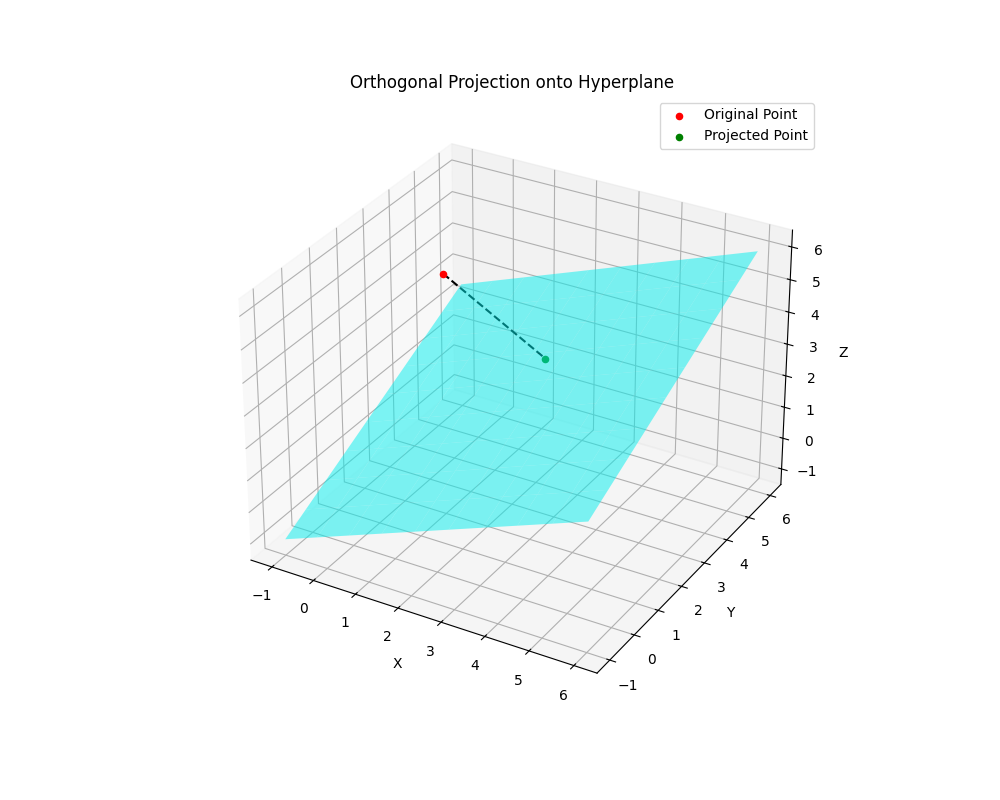
\includegraphics[width=0.6\linewidth]{illustrations/orthogonal_projection.png}
    \caption{$QQ^{T}$ projects vector $v$ to the hyperplane generated by the column vector of $Q$, i.e. $q_{1}=[1/\sqrt{3}, 1\sqrt{3}, 1\sqrt{3}]$ and $q_{2}=[1/\sqrt{2}, -1/\sqrt{2}, 0]$. For instance, point $[1\; 2\; 6]^{T}$ in red is projected to $[1.5\quad 2.5\quad 3]^{T}$}
    \label{fig:enter-label2}
\end{figure}


We need prepare some lemmas to be at bottom of simultaneous iteration, assume $V$ is matrix consisting of linearly independent columns $[v_{1}, v_{2}, \cdots, v_{k}]$ and we have the following proposition
\begin{Lemma}
\begin{enumerate}
    \item $V$ is injective is equivalent to $\widehat{V}$ is injective.
    
    \item $PV$ is injective is equivalent to $\widehat{P}\widehat{V}$ is injective.
    
    \item $PV$ is injective implies that $V$ is injective.
\end{enumerate}
    
\end{Lemma}

\begin{proof}
    The first can be easily proven by $v_{i} = Q Q^{*} v_{i} = Q\widehat{v}_{i}$. 

    We can view $PV$ as new matrix consisting of $w_{i}$ and find that $\widehat{PV} = \widehat{P} \widehat{V}$.
\end{proof}




\newpage
\section{Norms}
Since the norm of vector $x$ induces a metric space, one can see that the closed unit ball 
$$
\{x\in \mathbb{R}^{2}:\quad \|x\| = 1\}
$$
are different under different norm. Since the norm of matrix is defined by vector norm, it's worthwhile to give an illustration.

\begin{figure}[ht]
    \centering
    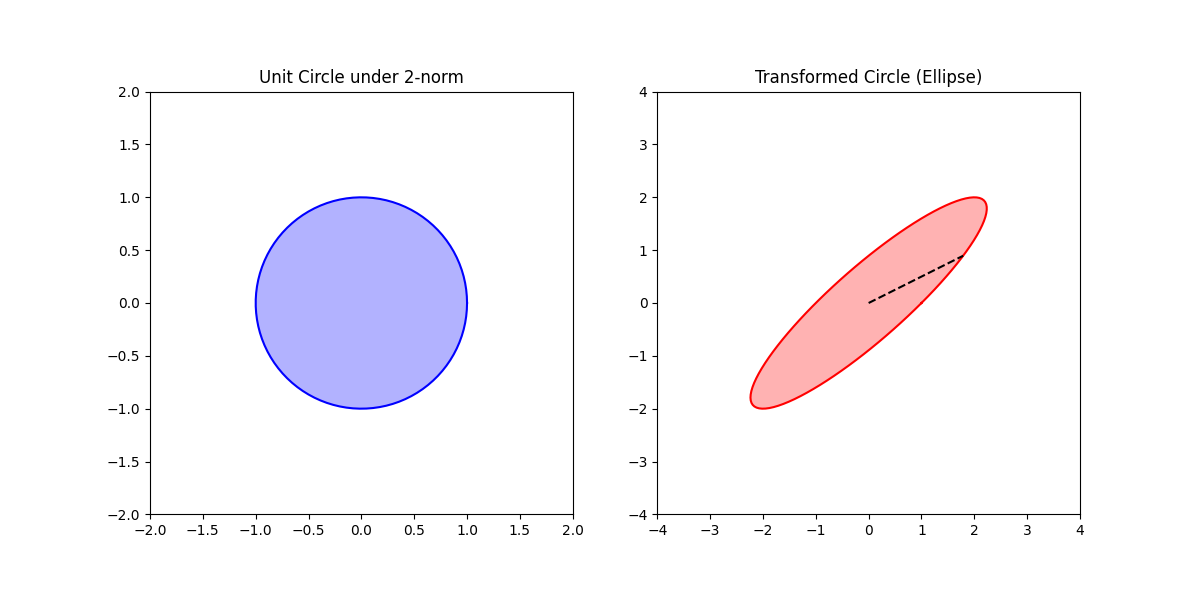
\includegraphics[width=1.0\linewidth]{illustrations/matrix_norm.png}
    \caption{The black dashed line is eigenvector of transformed matrix $[1 \;2; 0 \;2]$. The spectral of matrix $A$ is strictly less than $\|A\|$ since it's non-symmetric.}
    \label{fig:enter-label}
\end{figure}

\begin{problem}{}
    Let $\|\cdot\|$ denote any norm on $\mathbb{C}^m$ and also the induced matrix norm on $\mathbb{C}^{m \times m}$. Show that $\rho(A) \leq\|A\|$, where $\rho(A)$ is the spectral radius of $A$, i.e., the largest absolute value $|\lambda|$ of an eigenvalue $\lambda$ of $A$.
\end{problem}

\begin{proof}
    Suppose $\xi$ is one eigenvector corresponding to largest eigenvalue $\lambda$, then 
    $$
    x=\frac{\xi}{\|\xi\|}
    $$
    is a unit vector under $(\mathbb{C}^{m}, \|\cdot \|)$. 
    
    The conclusion comes from
    $$
    \|Ax\|=\| \lambda x\| = |\lambda| \|A\| =|\lambda| =\rho
    $$
    and $\|Ax\| \leq \|A\| \|x\| = \|A\|$. 
\end{proof}


\begin{Remark}
    Next, we show that 
    $$
    \rho(A) = \{\langle Ax,x\rangle, \|x\| = 1\} = \|A\|
    $$
    when $A$ is symmetric.

    By assumption, there is a unitary matrix $Q$ such that $Q^{*}AQ$ is a diagonal matrix with real number entry. Then
    $$
    \langle Ax,x\rangle = \langle QDQ^{*}x,x\rangle =\langle D\hat{x}, \hat{x}\rangle
    $$
    where $\hat{x}$ is the coordinates of $x$ under basis of $Q$. It's easy to see that $\lambda_{\min} \leq \langle Ax,x\rangle \leq \lambda_{\max}$. (Here we used the conclusion about unitary matrix $\|Qx\|=\|x\|$.)

    Next, we prove second equality, thanks to
    $$
    \langle Ax,Ax\rangle = \langle A^{*}Ax,x\rangle = \langle A^{2}x,x\rangle
    $$
    and the previous, we know that the maximum of $\langle Ax,Ax\rangle$ is $\lambda^{2}_{\max}$.
    
\end{Remark}

\begin{problem}{}
    Show that $\|A\| \leq \|A\|_{F}$.
\end{problem}

\begin{proof}
    This question reveals the importance of SYMMETRIC matrix.

    Suppose $A$ is symmetric, then by $A= QDQ^{T}$, one can see that $\|A\| = \lambda_{\max} < \|QDQ^{T}\|_{F}$.

    For general case, we have $\langle Ax, Ax\rangle = \langle A^{T}Ax, x\rangle$ where there is a symmetric matrix and one can deduce the conclusion easily once he
    notes that sum of diagonal elements of $A^{T}A$ is exactly the Frobenius norm of matrix $A$.
\end{proof}


\newpage

\section{Machine error and Roundoff}

\paragraph{Double precision.} 

\begin{Example}\label{example01}
    Take $x=9.4$ as an example, one can see it's stored in the following binary string
    \begin{equation}\label{eq01}
    +1.\fbox{$0010110011001100110011001100110011001100110011001101$}\times 2^3 .
    \end{equation}
\end{Example}
In computer arithmetic, the real number $x$ is replaced with the string of bits $\mathrm{fl}(x)$. According to this definition, $\mathrm{fl}(9.4)$ is the number in the binary representation \eqref{eq01}. We arrived at the floating point representation by discarding the infinite tail $. \overline{1100} \times 2^{-52} \times 2^3=. \overline{0110} \times 2^{-51} \times 2^3=.4 \times 2^{-48}$ from the right end of the number and then adding $2^{-52} \times 2^3=2^{-49}$ in the rounding step. Therefore,
$$
\begin{aligned}
\mathrm{fl}(9.4) & =9.4+2^{-49}-0.4 \times 2^{-48} \\
& =9.4+(1-0.8) 2^{-49} \\
& =9.4+0.2 \times 2^{-49} .
\end{aligned}
$$

In other words, a computer using double precision representation and the Rounding to Nearest Rule makes an error of $0.2 \times 2^{-49}$ when storing 9.4 . We call $0.2 \times 2^{-49}$ the rounding error. 

The important message is that the floating point number representing 9.4 is not equal to 9.4 , although it is very close. To quantify that closeness, we use the standard definition of error.

\begin{Definition}
    Let $x_{c}$ be computed version of the exact quantity $x$, then we call
    $$
    \frac{|x-x_{c}|}{x}
    $$
    the \textbf{relative error}.
\end{Definition}


\begin{Example}\label{example02}
    Continuing the example about $9.4$, one can see
    $$
    \frac{|\operatorname{fl}(9.4)-9.4|}{|9.4|}=\frac{0.2\times 2^{-49}}{9.4}=\frac{8}{47}\times 2^{-52}<\frac{1}{2}\mathbf{u}.
    $$
    where $\uu$ is machine epsilon.
\end{Example}

More general, one has
$$
\operatorname{fl}(a\circ b)=(a\circ b)(1+\delta), \quad \text{where}\; |\delta|< \uu.
$$
where $a\circ b$ is the operation between two numbers like $+,-,\times,/$.


\paragraph{Backward Stability.}
Algorithms in numerical linear algebra are usually classified from the point of view of the numerical stability as forward and backward stable. Say, that for some data $x$ you want to compute the solution $y$ given by some function $f: y=f(x)$. Because our world (and computers as well) is not ideal, we get some $\tilde{y}$ instead of $y$. We distinguish here between the forward error, that is, some norm of $y-\tilde{y}$ and backward error. 

The backward error answers the question of how much we have to perturb the input data $x$ for which we actually solved the problem, that is, we look for $\tilde{x}$ such that $\tilde{y}=f(\tilde{x})$. This problem is not usually uniquely solvable (there might be many $\tilde{x}$ satisfying this condition), so one usually seeks $\tilde{x}$ which is close to the original data $x$.


\newpage
\section{LU factorization}

\begin{problem}{}
    This is talking about backward stability in solving
$$
Ly=b
$$
where $L$ is $n\times n$ upper triangle matrix. Our algorithm is used to output $y$ after inputting $L$ and $b$, hence we want to find $\Delta L$ such that
\begin{equation}\label{eq02}
    (L+\Delta L)\tilde{y}=b
\end{equation}
\end{problem}

 
Assuming the simplest case
$$
l_{11}y_1=b_1,\quad (l_{11}+\Delta l_{11})\tilde{y}_{1}=b_1
$$
where $\tilde{y}$ is computed by forward substitution using machine. Subtract the first eq from the second, we get
$$
l_{11}(\tilde{y}-y)+\Delta l_{11}\tilde{y}=0,
$$
Hence
$$
\frac{|\Delta l_{11}|}{|l_{11}|}=\frac{|\tilde{y}-y|}{|\tilde{y}|} \leq \uu.
$$
where the last relative error about $\tilde{y}$ can be seen in Example \ref{example02}.

When $i\geq 2$, things becomes perplexing because there are more errors propagating in the process. In exact arithmetic, 
$$
l_{ii} y_{i}=b_{i}-\sum_{j=1}^{i-1}l_{ij}y_{j},\; i=1,2,\cdots,n.
$$
The algorithm in detail is
\begin{algorithm}
    \begin{algorithmic}[1]
    \For{$i=1$ to $n$, step 1}  
       \State $w^{(1)}\gets b_{i}$\;
        \For{$j=0$ to $i-1$, step 1}
           \State $w^{(j+1)}\gets w^{(j)}-l_{ij}y_{j}$ \;
        \EndFor
    \State $y_{i}\gets w^{(i)}/l_{ii}$\;
    \EndFor
    \end{algorithmic}
\end{algorithm}


There are two sources of error,
$$
\tilde{w}^{(j+1)}=\left(\tilde{w}^{(j)}-l_{i j} \tilde{y_j}\left(1+\delta_j\right)\right)\left(1+\delta_j^{\prime}\right), \quad\left|\delta_j\right| \leq \uu, \quad\left|\delta_j^{\prime}\right| \leq \uu
$$
and
$$
l_{i i} \tilde{y_i}=\left(1+\delta_i\right) \tilde{w}^{(i)}, \quad\left|\delta_i\right| \leq \uu .
$$

Putting these together gives
$$
\frac{l_{i i} \tilde{y_i}}{1+\delta_i}=b_i\left(1+\delta_1^{\prime}\right) \cdots\left(1+\delta_{i-1}^{\prime}\right)-\sum_{j=1}^{i-1} l_{i j} \tilde{y_j}\left(1+\delta_j\right)\left(1+\delta_j^{\prime}\right) \cdots\left(1+\delta_{i-1}^{\prime}\right)
$$
and dividing by the factor in the term containing $b_i$ leads to
\begin{equation}\label{eq03}
    \frac{l_{i i} \tilde{y_i}}{\left(1+\delta_i\right)\left(1+\delta_1^{\prime}\right) \cdots\left(1+\delta_{i-1}^{\prime}\right)}=b_i-\sum_{j=1}^{i-1} l_{i j} \tilde{y_j} \frac{1+\delta_j}{\left(1+\delta_1^{\prime}\right) \cdots\left(1+\delta_{j-1}^{\prime}\right)}
\end{equation}

Comparing eq\eqref{eq03} with our goal eq\eqref{eq02} written as followings
$$
\sum_{j\leq i} (l_{ij}+\Delta l_{ij})\tilde{y}_{j}=b_{i},
$$
we deduce 
$$
\tilde{l}_{i i}=\frac{l_{i i}}{\left(1+\delta_i\right)\left(1+\delta_1^{\prime}\right) \cdots\left(1+\delta_{i-1}^{\prime}\right)}=\left(1+\epsilon_{i i}\right) l_{i i}, \quad\left|\epsilon_{i i}\right| \leq i \uu+O\left(\uu^2\right)
$$
and
$$
\tilde{l}_{i j}=\frac{l_{i j}\left(1+\delta_j\right)}{\left(1+\delta_1^{\prime}\right) \cdots\left(1+\delta_{j-1}^{\prime}\right)}=l_{i j}\left(1+\epsilon_{i j}\right), \quad\left|\epsilon_{i j}\right| \leq j \uu+O\left(\uu^2\right) .
$$


\newpage

\section{QR Decomposition}

In this section, we investigate QR factorization and Householder reflection.
Just like LU factorization, we view QR factorization as \textbf{encoding} following process
$$
AR^{-1}=Q
$$
i.e. manipulating the columns of $A$ to get orthogonal matrix.

First, we investigate the algorithm derived from Grad-Schmit

\begin{algorithm}
    \begin{algorithmic}[1]
    \Require{$m\times n$ matrix $A$}
    \For{$i=1$ to $n$}  
        \State $q_{i} \gets A(1:m;i)$
        \For{$j=1$ to $i-1$}
           \State $r_{ji}\gets A(1:m;j)^{T}q_{i}$ \;
           \State $q_{i}=q_{i}-r_{ji} A(1:m;j)$ \;
        \EndFor
    \State $A(1:m;i)\gets q_{i}/\|q_{i}\|_{2}^{2}$\;
    \EndFor
    \end{algorithmic}
\end{algorithm}


\begin{Example}\label{example03}
    This is about the stability of QR factorization.

    We have seen the example like when $\delta=10^{-10}$ and 
    $$
    A=\left[\begin{array}{ccc}
    1 & 1 & 1\\
    \delta &0 &0 \\
    0 & \delta & 0\\
    0 & 0& \delta
    \end{array}\right].
    $$
    One have to understand that one discard $\varepsilon$ in the process of roundoff 
    $$
    \operatorname{fl}(1+\delta^{2})=1,
    $$
    while one cannot view $\sqrt{\delta^{2}+\delta^{2}}$ as 0. That's why we call $10^{-15}$ as relative representation error and $[10^{-308}, 10^{308}]$ is the range of double precision.
\end{Example}




Next, we use Householder reflector to realize QR factorization, where we use orthogonal matrix $Q$ to put zeros in $a_{ij},i>j$, in other words, we view $A=QR$ as
$$
Q^{-1}A=Q^{-1}[\alpha_{1}\mid \alpha_{2} \mid\cdots \mid\alpha_{n}]=R.
$$
Therefore we need find an orthogonal matrix $Q^{-1}$ such that $Q^{-1}\alpha_{1}=ce_{1}$ and if we can do this, we can use the same pattern to finish the factorization. (induction idea is very common!)



\begin{Remark}
    I realized the QR algorithm \cite{trefethen2022numerical}[Algorithm 10.1, 10.3] in Python, which is very worthwhile. I learned some points like
    \begin{itemize}
        \item $(I-2qq^{*})v$ can be executed as $v - 2q(q^{*}v)$ which avoids multiplication between matrix $qq^{*}$ and vector $v$.
        
        \item Count computational cost: first find the predominant part and analyze the flops per capita!

        \item Implicit calculation of a product $Qx$.
    \end{itemize}
\end{Remark}


\newpage
\section{Eigenvalue and Eigenvector}

Here I state a result which will be used again and again in the following text.

\begin{problem}{}
     Suppose $A, E \in \mathbb{C}^{n \times n}$ are self-adjoint with eigenvalues $\lambda_1 \geq \cdots \geq \lambda_n, \epsilon_1 \geq \cdots \geq \epsilon_n$ respectively, and $B=A+E$ has eigenvalues $\mu_1 \geq \cdots \geq \mu_n$. Prove that $\lambda_i+\epsilon_1 \geq \mu_i \geq \lambda_i+\epsilon_n$
\end{problem}

\begin{proof}
    When eigenvalues of self-adjoint matrix $A$ are arranged in descending order (from large to small), we have
    $$
    \lambda_{k} = \max_{\operatorname{dim}(V) = k} \min_{v\in V} \langle Av, v\rangle.
    $$
    When eigenvalues are arranged in ascending order, we have
    $$
    \mu_{k} = \min_{\operatorname{dim}(V) = n-k+1} \max \langle Av, v\rangle.
    $$

    Taking the above statement for granted, we now prove $\mu_{i} \leq \lambda_{i} + \epsilon_{1}.$

    $$
    \begin{aligned}
        \mu_{i} & =\min_{\operatorname{dim}(V) = n-i+1} \max_{v} \left(v^{*}(A+E) v\right)\\
        & \leq \min_{\operatorname{dim}(V) = n-i+1} \left(\max_{v} v^{*}Av +\max_{v} v^{*}Ev\right)\\
        &\leq \lambda_{i} + \epsilon_{1}.
    \end{aligned}
    $$
\end{proof}
 


\subsection{Jacobi Iteration}

\begin{problem}{}
    Write a program to find the eigenvalues of an $m \times m$ real symmetric matrix by the Jacobi algorithm with the standard row-wise ordering, plotting the sum of the squares of the off-diagonal entries on a log scale as a function of the number of sweeps. Apply your program to random matrices of dimensions 20,40 , and 80 .
\end{problem}





\subsection{Power Method}
Let me brush up the main points in \cite{borm2012numerical}. 


\subsection*{Rayleigh Quotient}
Assume we get a vector $v^{(k)}$ after $k$-step iterations, then we face the problem in solving approximate eigenvalue $x$, i.e. 
$$
x v=Av
$$
Numerically, $Av$ and $v$ are not parallel and this boils down to solving inconsistent linear system. One can apply the conclusion of Least Square to get \textbf{Rayleigh quotient}:
\begin{equation}
    \label{RayleighQ}
    x = \Lambda_{A}(v) := \frac{v^{*}Av}{v^{*}v}
\end{equation}
Also one can get the same result\eqref{RayleighQ} by solving the following optimization problem
\begin{equation}
    \label{optimization1}
    \operatorname{min}_{x} \|Av-x v\|_{2}^{2}
\end{equation}

Geometrically, one find a scalar $x$ such that $Av-xv$ is orthogonal to $v$. Algebraically, eq\eqref{optimization1} (take real case as example) boils down to find the critical point of
$$
f(x)=v^{T}v ^{2}- v^{T}(A^{T}+A)v x+v^{T}A^{T}Av
$$
If $v^{T}A^{T}v$ is real number, then $v^{T}A^{T}v = v^{T}Av$, one can use derivative of $f(x)$ to determine the critical point and the result matches the Least Square. When we consider complex number field, the expansion of $f(x)=\operatorname{min}_{x} \|Av-x v\|_{2}^{2}$ is subtle, saying
$$
f(x)\neq v^{*}v x^{2}- v^{*}(A^{*}+A)v x+v^{*}A^{*}Av
$$
especially $x$ is complex. 

\paragraph{Residue Analysis}
Based on the analysis above, there are orthogonal vectors $v$ and $xv-Av$ and this offers a way to create a self adjoint matrix $B$ such that $v$ is exactly the eigenvector of $B$, which means little difference between $A$ and $B$.

Review example\ref{example04}, one knows that $vr^{*} +r v^{*}$ is a self-adjoint matrix sending $v$ to $r=xv-Av$. We can add this matrix by $A$ to eliminate $Av$, which yields $B=vr^{*} +r v^{*}+A$.

When considering simultaneous iteration to get invariant subspace (eigenvector space), the difference between theory and practice appears. For example
\subsection*{Numerical Instability and Orthogonalization}


Consider the symmetric matrix:

$$
A = \begin{bmatrix} 4 & 1 & 1 \\ 1 & 3 & 1 \\ 1 & 1 & 2 \end{bmatrix}
$$

We will start with the matrix $V$ with two columns in the initial step:

$$
V^{(0)} = \begin{bmatrix} 1 & 0 \\ 0 & 1 \\ 0 & 0 \end{bmatrix}
$$

\subsubsection*{Iteration Without Orthogonalization}

Each column of $ V^{(m)} $ is updated via:
$$
V^{(m+1)} = A V^{(m)}
$$

Perform a few iterations to illustrate the convergence:

\paragraph{First Iteration:}

$$
V^{(1)} = A V^{(0)} = \begin{bmatrix} 4 & 1 & 1 \\ 1 & 3 & 1 \\ 1 & 1 & 2 \end{bmatrix} \begin{bmatrix} 1 & 0 \\ 0 & 1 \\ 0 & 0 \end{bmatrix} = \begin{bmatrix} 4 & 1 \\ 1 & 3 \\ 1 & 1 \end{bmatrix}
$$

\paragraph{Second Iteration:}

$$
V^{(2)} = A V^{(1)} = \begin{bmatrix} 4 & 1 & 1 \\ 1 & 3 & 1 \\ 1 & 1 & 2 \end{bmatrix} \begin{bmatrix} 4 & 1 \\ 1 & 3 \\ 1 & 1 \end{bmatrix} = \begin{bmatrix} 18 & 8 \\ 8 & 11 \\ 7 & 6 \end{bmatrix}
$$

\paragraph{... 10th Iteration:}

$$
V^{(10)} = A V^{(9)} = \begin{bmatrix} 8490718 & 5843148 \\ 5843148 & 4032371 \\ 4458347 & 3073546 \end{bmatrix}
$$

\subsubsection*{Observation}

As iterations continue, each column increasingly aligns with the dominant eigenvector $\mathbf{v}_1 = \begin{bmatrix} 0.7558 \\ 0.5207 \\ 0.3971 \end{bmatrix}$ corresponding to $\lambda_{\max} = 5.2143$. For large $ m $, the columns of $ V^{(m)} $ converge to:

$$
V^{(m)} \approx \begin{bmatrix} 0.7558 & 0.5207 \\ 0.3971 & 0.7558 \\ 0.5207 & 0.3971 \end{bmatrix}
$$

This convergence indicates numerical instability, as the columns lose linear independence and all vectors converge toward the dominant eigenvector's direction.

\subsubsection*{Apply QR into Simultaneous Iteration}

\paragraph{Orthogonalize (using QR Factorization):}

Perform QR factorization when computing $V^{(2)}= AV^{(1)} = A$ where
$$
V^{(1)} = \begin{bmatrix} 4 & 1 \\ 1 & 3 \\ 1 & 1 \end{bmatrix} =Q^{(1)}R^{(1)}=  \begin{bmatrix}
-0.9428 & 0.2851 \\
-0.2357 & -0.9366 \\
-0.2357 & -0.2036
\end{bmatrix} \begin{bmatrix}
-4.2426 & -1.8856 \\
0 & -2.7285
\end{bmatrix}
$$,
then we compute the QR of $AQ^{(1)} = Q^{2} \hat{R}^{(2)}$,

$$
\begin{aligned}
    V^{(2)}& =Q^{(2)} \hat{R}^{(2)}R^{(1)}\\
            & = \begin{bmatrix}
-0.8611 & 0.4685 \\
-0.3827 & -0.8531 \\
-0.3349 & -0.2297
\end{bmatrix} \begin{bmatrix}
4.9272 & 1.3987 \\
0 & 2.5708
\end{bmatrix}\begin{bmatrix}
-4.2426 & -1.8856 \\
0 & -2.7285
\end{bmatrix}
\end{aligned}
$$

\paragraph{Update $V^{(m)}$ with orthogonal columns:} 

After orthogonalization:
$$
V^{(m)}=Q^{(m)} R^{(m)} =\begin{pmatrix}
-0.7559 & 0.6316 \\
-0.5205 & -0.7395 \\
-0.3971 & -0.2330
\end{pmatrix} 1.0e+07 \begin{pmatrix}
-5.8556 & -4.0339 \\
0 & -0.0024
\end{pmatrix}
$$
with $m = 10$ as example. One can verify that the columns of $Q^{(10)}$ closely approximate the eigenvectors of $A$ corresponding to its two largest eigenvalues (in magnitude).

This orthogonalization corrects the numerical errors that lead to loss of linear independence, thus ensuring each iteration step mainly jumps to the invariant subspace.





\subsection{QR Iteration}
The QR method mentioned to compute eigenvalues has some points which can be improved. For example,


\subsection{Improved QR Iteration}

\newpage
\section{Exercise}
\begin{problem}{}
    Let $A \in \mathbb{R}^{n \times n}$ and $S \in \mathbb{R}^{r \times r}, r<n$, be symmetric matrices such that
    \begin{equation}
    \label{eq_ex01}
        A Q_1-Q_1 S=E_1
    \end{equation}
    where $Q_1 \in \mathbb{R}^{n \times r}$ and $Q_1^T Q_1=I$. Show that, there exist $\mu_1, \cdots, \mu_r \in \lambda(A)$ such that
    
    $$
    \left|\mu_k-\lambda_k(S)\right| \leq \sqrt{2}\left\|E_1\right\|_2, \quad k=1, \cdots, r
    $$
    
    where $\lambda(B)$ denotes the set of all eigenvalues of $B$.
\end{problem}

A natural way to deal with non-square isometric matrix is to extend it. Suppose $Q = [Q_{1} \;\;Q_{2}]$ is $n\times n$ isometric and then $Q^{T} AQ$ is similar to $A$ and has the same eigenvalue. We can write $Q^{T}A Q$ into block form, i.e.
$$
\begin{aligned}
\begin{bmatrix}
     Q_{1}^{T}  \\
     \\
     Q_{2}^{T} 
\end{bmatrix} A
\begin{bmatrix}
    Q_{1} & Q_{2}
\end{bmatrix} &= \begin{bmatrix}
     Q_{1}^{T} A \\
     \\
     Q_{2}^{T} A
\end{bmatrix}\begin{bmatrix}
    Q_{1} & Q_{2}
\end{bmatrix}\\
& = \begin{bmatrix}
    Q_{1}^{T}AQ_{1} & Q_{1}^{T}AQ_{2}\\
    \\
    Q_{2}^{T} A Q_{1} & Q_{2}^{T}AQ_{2}
\end{bmatrix}\\
& = \begin{bmatrix}
    S & \\
    \\
     & Q_{2}^{T}A Q_{2}
\end{bmatrix} + \begin{bmatrix}
    Q_{1}^{T} E_{1} & Q_{1}^{T}AQ_{2}\\
    \\
    Q_{2}^{T} A Q_{1} & O
\end{bmatrix}
\end{aligned}
$$

where the first equation comes from the following rule of block matrix: assume we split matrix $M$ into upper and lower block with the same number of columns, then 
$$
Mx = \begin{bmatrix}
    M_{1:k, 1:n}\\
    \\
    M_{k+1:n, 1+n}
\end{bmatrix}x = \begin{bmatrix}
    M_{1:k, 1:n}x\\
    \\
    M_{k+1:n, 1+n}x
\end{bmatrix}
$$
This can be interpreted as we split a system of $n$ equations into two system of equations (in formal).


By the equation of $Q^{T}AQ$, we know that the difference of $|\mu -\lambda|$ can be controlled by the norm of matrix
$$
\begin{bmatrix}
    Q_{1}^{T} E_{1} & Q_{1}^{T}AQ_{2}\\
    \\
    Q_{2}^{T} A Q_{1} & O
\end{bmatrix} =\begin{bmatrix}
    Q_{1}^{T} E_{1} & E_{1}^{T} Q_{2}\\
    \\
    Q_{2}^{T} E_{1} & O
\end{bmatrix},
$$
where we use the property $Q_{2}^{T} Q_{1} = O$ and assumed equation\eqref{eq_ex01}

Let's derive the bound in the following.

$$
E = \begin{bmatrix} 
Q_1^T E_1 & E_1^T Q_2 \\
\\ 
Q_2^T E_1 & 0 \end{bmatrix}, \quad y = 
\begin{bmatrix} \hat{y} \\
\\ 
y_\perp \end{bmatrix}
$$

Then:

$$
Y = Ey = \begin{bmatrix} 
Q_1^T E_1 \hat{y} + E_1^T Q_2 y_\perp \\
\\
Q_2^T E_1 \hat{y} \end{bmatrix}
$$

The squared norm of $Y$ is:

$$
\|Y\|^2 = \|Q_1^T E_1 \hat{y} + E_1^T Q_2 y_\perp\|^2 + \|Q_2^T E_1 \hat{y}\|^2
$$

Using the triangle inequality:

$$
\|Y\|^2 \le (\|Q_1^T E_1 \hat{y}\| + \|E_1^T Q_2 y_\perp\|)^2 + \|Q_2^T E_1 \hat{y}\|^2
$$

Using $(a+b)^2 \le 2(a^2 + b^2)$:

$$
\|Y\|^2 \le 2(\|E_1\|^2 \|\hat{y}\|^2 + \|E_1\|^2 \|y_\perp\|^2) + \|E_1\|^2 \|\hat{y}\|^2
$$

Since $\|y\|^2 = \|\hat{y}\|^2 + \|y_\perp\|^2$:

$$
\|Y\|^2 \le 2\|E_1\|^2 \|y\|^2 + \|E_1\|^2 \|\hat{y}\|^2 \le 3\|E_1\|^2 \|y\|^2
$$

Therefore:

$$
\|Y\| \le \sqrt{3} \|E_1\| \|y\|
$$

This implies:

$$
\|E\| \le \sqrt{3} \|E_1\|
$$

Therefore, the best bound we can obtain with this approach is $\sqrt{3}\|E_1\|$.  To achieve $\sqrt{2}\|E_1\|$ would require additional assumptions or a different approach.
Final Answer: The final answer is $\boxed{\sqrt{3}||E_1||}$

 



\bibliography{reference} % The name of your .bib file without the .bib extension
\end{document}

